% Options for packages loaded elsewhere
\PassOptionsToPackage{unicode}{hyperref}
\PassOptionsToPackage{hyphens}{url}
%
\documentclass[
]{article}
\usepackage{amsmath,amssymb}
\usepackage{lmodern}
\usepackage{iftex}
\ifPDFTeX
  \usepackage[T1]{fontenc}
  \usepackage[utf8]{inputenc}
  \usepackage{textcomp} % provide euro and other symbols
\else % if luatex or xetex
  \usepackage{unicode-math}
  \defaultfontfeatures{Scale=MatchLowercase}
  \defaultfontfeatures[\rmfamily]{Ligatures=TeX,Scale=1}
\fi
% Use upquote if available, for straight quotes in verbatim environments
\IfFileExists{upquote.sty}{\usepackage{upquote}}{}
\IfFileExists{microtype.sty}{% use microtype if available
  \usepackage[]{microtype}
  \UseMicrotypeSet[protrusion]{basicmath} % disable protrusion for tt fonts
}{}
\makeatletter
\@ifundefined{KOMAClassName}{% if non-KOMA class
  \IfFileExists{parskip.sty}{%
    \usepackage{parskip}
  }{% else
    \setlength{\parindent}{0pt}
    \setlength{\parskip}{6pt plus 2pt minus 1pt}}
}{% if KOMA class
  \KOMAoptions{parskip=half}}
\makeatother
\usepackage{xcolor}
\usepackage[margin=1in]{geometry}
\usepackage{graphicx}
\makeatletter
\def\maxwidth{\ifdim\Gin@nat@width>\linewidth\linewidth\else\Gin@nat@width\fi}
\def\maxheight{\ifdim\Gin@nat@height>\textheight\textheight\else\Gin@nat@height\fi}
\makeatother
% Scale images if necessary, so that they will not overflow the page
% margins by default, and it is still possible to overwrite the defaults
% using explicit options in \includegraphics[width, height, ...]{}
\setkeys{Gin}{width=\maxwidth,height=\maxheight,keepaspectratio}
% Set default figure placement to htbp
\makeatletter
\def\fps@figure{htbp}
\makeatother
\setlength{\emergencystretch}{3em} % prevent overfull lines
\providecommand{\tightlist}{%
  \setlength{\itemsep}{0pt}\setlength{\parskip}{0pt}}
\setcounter{secnumdepth}{-\maxdimen} % remove section numbering
\ifLuaTeX
  \usepackage{selnolig}  % disable illegal ligatures
\fi
\IfFileExists{bookmark.sty}{\usepackage{bookmark}}{\usepackage{hyperref}}
\IfFileExists{xurl.sty}{\usepackage{xurl}}{} % add URL line breaks if available
\urlstyle{same} % disable monospaced font for URLs
\hypersetup{
  pdftitle={Lista 1 - Exercício B},
  pdfauthor={Gustavo Tironi},
  hidelinks,
  pdfcreator={LaTeX via pandoc}}

\title{Lista 1 - Exercício B}
\author{Gustavo Tironi}
\date{10/05/2023}

\begin{document}
\maketitle

{
\setcounter{tocdepth}{2}
\tableofcontents
}
\hypertarget{escolha-do-gruxe1fico}{%
\section{Escolha do gráfico}\label{escolha-do-gruxe1fico}}

Inicialmente, a partir do material disponibilizado no \textbf{ECLASS}
achei interessante o gráfico do Willian Playfair então pesquisei na
internet e achei o um gráfico feito em R, disponivel
\href{https://github.com/carloscinelli/Blog-Scripts}{aqui} e mostrado a
seguir:

\includegraphics{lista1_c_files/figure-latex/unnamed-chunk-1-1.pdf}

Vale pontuar que foram necessárias algumas mudanças no código original
para que funcionasse corretamente, já que o mesmo contêm uma fonte de
texto a qual não obtive acesso e possui alguns comando que mudaram nas
versões mais recentes do R.

\hypertarget{modificando-o-gruxe1fico}{%
\section{Modificando o gráfico}\label{modificando-o-gruxe1fico}}

Inicialmente, pensei em mudar o eixo para direita, pois é assim que o
gráfico original é apresentado. Fiz isso, usando o seguinte código:

\begin{verbatim}
scale_y_continuous(position = "right")
\end{verbatim}

Após isso, resolvi arrumar também a escala do eixo y, já que o original
inicia do 0, enquanto o plotado em R começa do 30. Para isso, utilizei o
seguinte comando:

\begin{verbatim}
scale_y_continuous(limits = c(10000, NA))
\end{verbatim}

Após isso, fiz varias mudanças menores, como mudança no \textbf{título},
na \textbf{largura da linha}, na \textbf{posição dos textos} e nas
\textbf{cores}. Ficando com o seguinte gráfico ao final das mudanças:

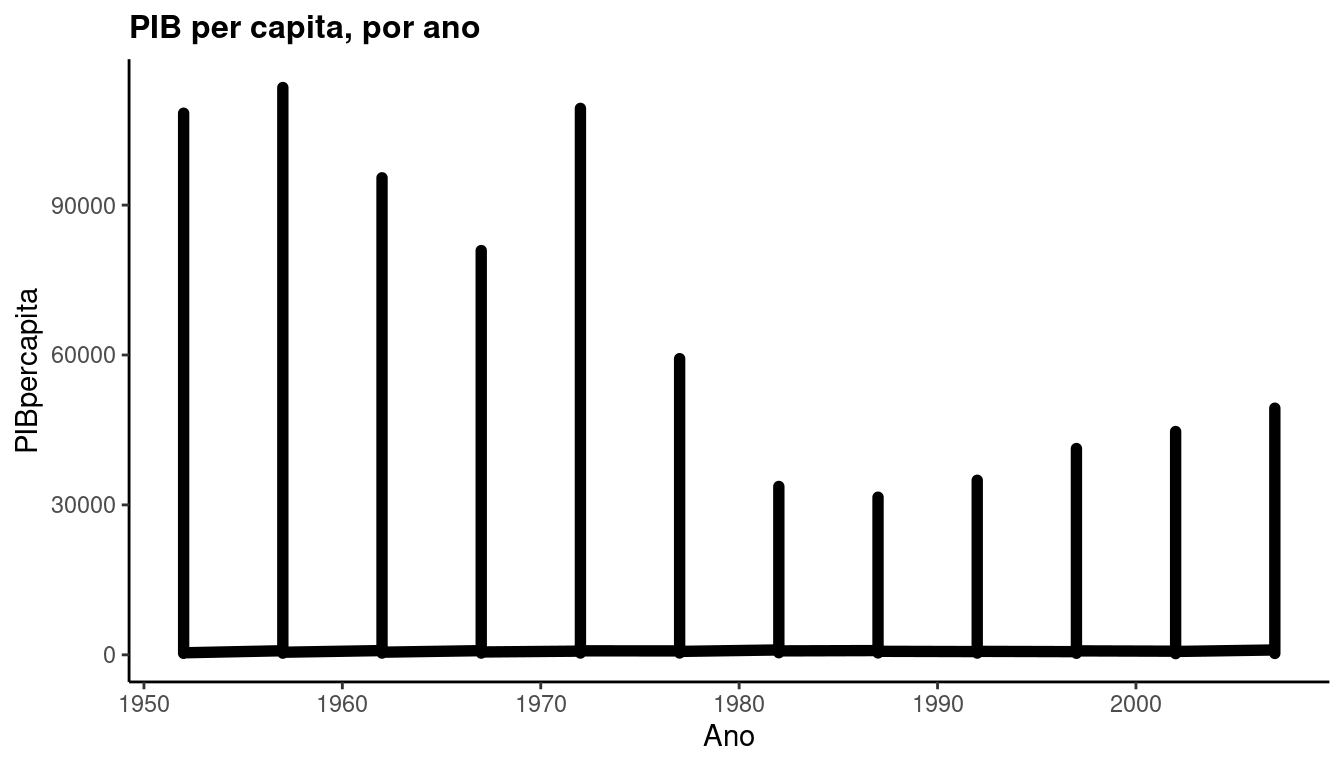
\includegraphics{lista1_c_files/figure-latex/unnamed-chunk-2-1.pdf}

Por fim, resolvi adiconar informações ao gráfico, apenas com o fim de
aprender alguns comandos novos em R. Então resolvi adicionar
\textbf{linhas verticais} que separam o gráfico pelos reis que
governavam em cada periodo. Para isso, eu precisava adicionar as
\textbf{linhas verticais} nas datas adequadas, e indicar com um
\textbf{texto} qual rei governava o periodo. Para adicionar as linhas
adicionei variaçẽos do seguinte comando:

\begin{verbatim}
geom_vline(xintercept = (data de mudança do reinado), linetype = "dashed")
\end{verbatim}

Agora para adicionar os textos, usei um comando que já tinha sido usado
pelo autor original do gráfico, que é o \textbf{annotate}, variando os
seus parametros. Ao final, o resultado foi o seguinte:

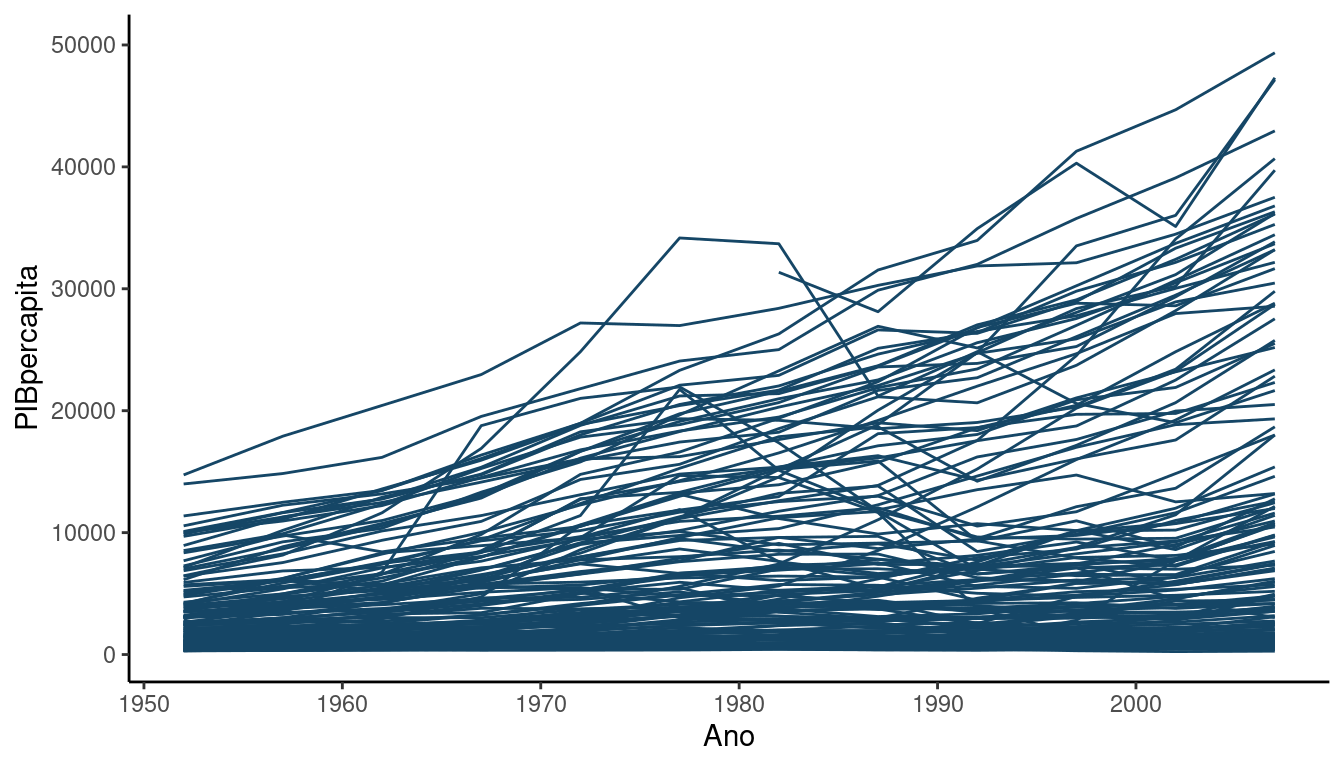
\includegraphics{lista1_c_files/figure-latex/unnamed-chunk-3-1.pdf}

Sendo o código final o seguite:

\begin{verbatim}
library(reshape2)
library(ggplot2)
library(stats)

playfair <- readRDS("william_playfair.rds")

playfair$min <- with(playfair, pmin(exp, imp))
year <- playfair$year

molten_data <- melt(playfair,  id.vars = c("year", "min"))

ggplot(molten_data, aes(x = year, y = value)) + 
  geom_line(aes(col = variable), size  = 1.1) +
  geom_ribbon(aes(ymin = min, ymax = value, fill = variable), alpha = 0.3) +
  scale_color_manual(values = c("darkred", "gold3"), guide = "none") + 
  scale_fill_manual(values = c("#90752d", "#BB5766"), guide = "none") + 
  theme_bw() + 
  annotate("text", x = year[5],        y = 101000, label = "Line", angle = 25, size = 3) +
  annotate("text", x = year[6] - 100,  y = 105000, label = "of",  angle = 0, size = 3) +
  annotate("text", x = year[7],        y = 102000, label = "Imports", angle = 340, size = 3) +
  annotate("text", x = year[5] + 400,  y = 72000,  label = "Line",  angle = 345, size = 3) +
  annotate("text", x = year[6],        y = 69000,  label = "of",  angle = 330, size = 3) +
  annotate("text", x = year[7] - 200,  y = 62400,  label = "Exports",  angle = 335, size = 3) +
  annotate("text", x = year[8]+150,        y = 83000,  label = 'BALANCE AGAINST',  angle = 0, fontface = "bold.italic") +
  annotate("text", x = year[16] + 400, y = 110000, label = 'BALANCE in\nFAVOUR of\nENGLAND',  angle = 0, fontface = "bold.italic") +
  annotate("text", x = year[16],       y = 80800,  label = "Imports",  angle = 20, size = 3) +
  annotate("text", x = year[14] + 100, y = 131000, label = "Exports",  angle = 55, size = 3) +
  annotate("text", x = year[4],  y = 145000,  label = "Frederick IV", size = 6) +
  annotate("text", x = year[8]+1100,  y = 145000,  label = "Christian VI", size = 6) +
  annotate("text", x = year[12]+200,  y = 165000,  label = "Frederick V", size = 6) +
  annotate("text", x = year[17],  y = 45000,  label = "Christian VII", size = 6) +
  ggtitle("Exports and Imports to and from DENMARK & NORWAY from 1700 to 1780") + 
  scale_x_date(breaks = seq(year[1], year[18], by = "10 years"), 
               labels = format(seq(year[1], year[18], by = "10 years"), "%Y")) + 
  scale_y_continuous(breaks = seq(0, 190e3, 10e3), 
                     labels = seq(0, 190, 10),
                     position = "right",
                     limits = c(10000, NA)) +
  theme(title = element_text(size = 12, face = 'bold'),
        plot.title = element_text(hjust=0.5),
        axis.title = element_blank(),
        axis.text = element_text(), 
        panel.grid.minor = element_blank(),
        panel.grid.major = element_line(color = "#c8c8c6"),
        panel.background = element_rect(fill = "#fcfcfa")) +
  geom_vline(xintercept = year[7], linetype = "dashed") +
  geom_vline(xintercept = year[10]+300, linetype = "dashed") +
  geom_vline(xintercept = year[15]+100, linetype = "dashed")
\end{verbatim}

\end{document}
